\documentclass[tikz,border=6pt]{standalone}
\usetikzlibrary{arrows.meta,positioning,calc}
\usepackage{pgfplots}

\begin{document}
\begin{tikzpicture}[>=Latex, font=\small]

% ---------- layout ----------
\def\panelW{7.0cm}
\def\panelH{4.2cm}
\def\xgap{9.9cm} % increased spacing
\def\ygap{7.2cm}  % increased spacing

% anchors (centers of each panel area)
\coordinate (UL) at (-0.15,\ygap);
\coordinate (BL) at (0,0);
\coordinate (UR) at (\xgap,\ygap);
\coordinate (BR) at (\xgap,0);

% titles (remove if not needed)
\node[above=18mm of UL] {Inverse CDF $F_t^{-1}(p)$};
\node[above=18mm of UR] {Inverse CDF $F_{t+T}^{-1}(p)$};

% styles
\tikzset{
  axisline/.style={line width=0.8pt},
  curve/.style={line width=1.2pt},
  arr/.style={->, line width=1.2pt},
  barfill/.style={fill=black!12, draw=black!60}
}

%%%%%%%%%%%%%%%%%%%%%%%%%%%%
% Upper-left: monotone ICDF
%%%%%%%%%%%%%%%%%%%%%%%%%%%%
\begin{scope}[shift={(-2,5)}]

  % ICDF definition
  \pgfmathdeclarefunction{Q}{1}{%
    \pgfmathparse{(#1)^3}%
  }

  % Evaluate endpoints for dashed guides
  \pgfmathparse{Q(-1)} \let\Qminus\pgfmathresult
  \pgfmathparse{Q( 1)} \let\Qplus \pgfmathresult

  \begin{axis}[
    width=5.4cm, height=6.2cm,
    xmin=-1, xmax=1,
    ymin={min(0,\Qminus)-0.10*abs(\Qplus-\Qminus)},
    ymax={\Qplus + 0.10*abs(\Qplus-\Qminus)},
    axis x line=bottom,        % only the x-axis at the bottom
    axis y line=none,          % no y-axis
    axis line style={-},       % <-- ensure no arrowheads
    xlabel={$p$}, ylabel={},
    xtick=\empty, ytick=\empty,
    xlabel style={yshift=8pt},
    clip=false
  ]

    % ICDF curve
    \addplot[very thick, domain=-1:1, samples=400] ({x},{Q(x)});

    % short vertical ticks + labels at p=-1 and p=1
    \node[draw=none] at (0, -20)   (a) {$-1$};
    \node[draw=none] at (200, -20)   (b) {$1$};

    % dashed verticals from curve endpoints down to x-axis
    \draw[dashed] (axis cs:-1,-1.2) -- (axis cs:-1,\Qminus);
    \draw[dashed] (axis cs: 1,-1.2) -- (axis cs: 1,\Qplus);

  \end{axis}

\end{scope}

%%%%%%%%%%%%%%%%%%%%%%%%%%%%%%%%%%%%%%%%%%%%%
% Bottom-left: histogram (from ICDF samples)
%%%%%%%%%%%%%%%%%%%%%%%%%%%%%%%%%%%%%%%%%%%%%
\begin{scope}[shift={(-2.9,-3)}] % move/scale/rotate the whole panel here
  \node[anchor=south west, inner sep=0, scale=0.7] (img) at (0,0)     {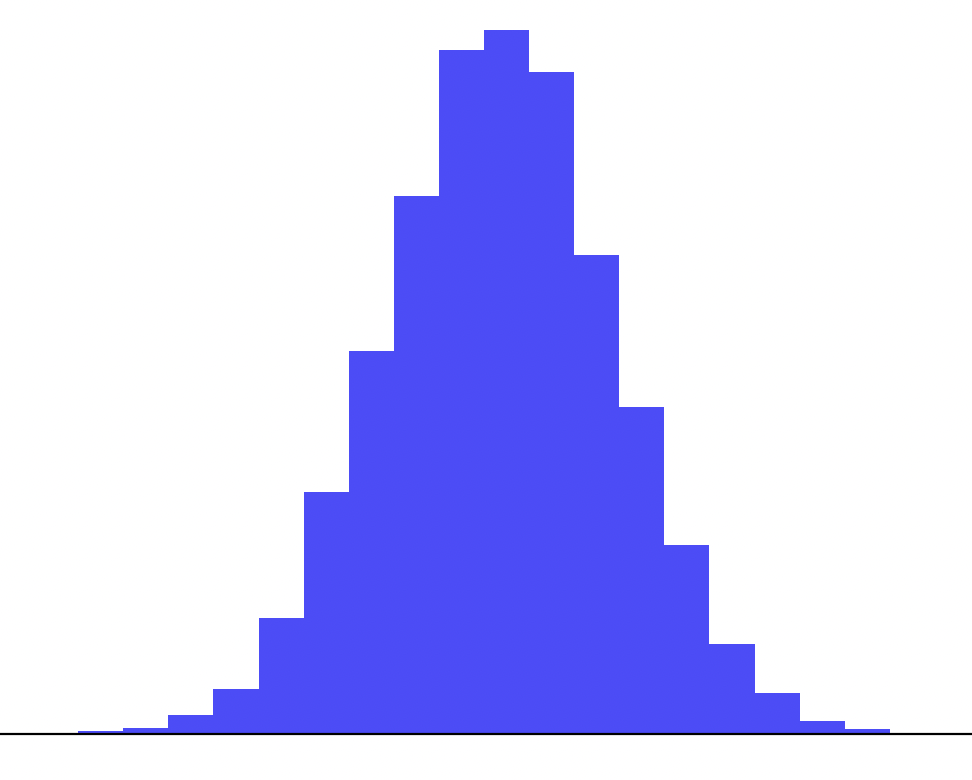
\includegraphics[width=8cm]{figures/hist1.png}};
  \node[draw=none] at (2.9,0.) {$X_t$};
\end{scope}

%%%%%%%%%%%%%%%%%%%%%%%%%%%%%%%%%%%%%%%%%%%%%
% Bottom-right: histogram after timestepper
%%%%%%%%%%%%%%%%%%%%%%%%%%%%%%%%%%%%%%%%%%%%%
\begin{scope}[shift={(7.5,-2.9)}] % move/scale/rotate the whole panel here
  \node[anchor=south west, inner sep=0, scale=0.68] (img) at (0,0)     {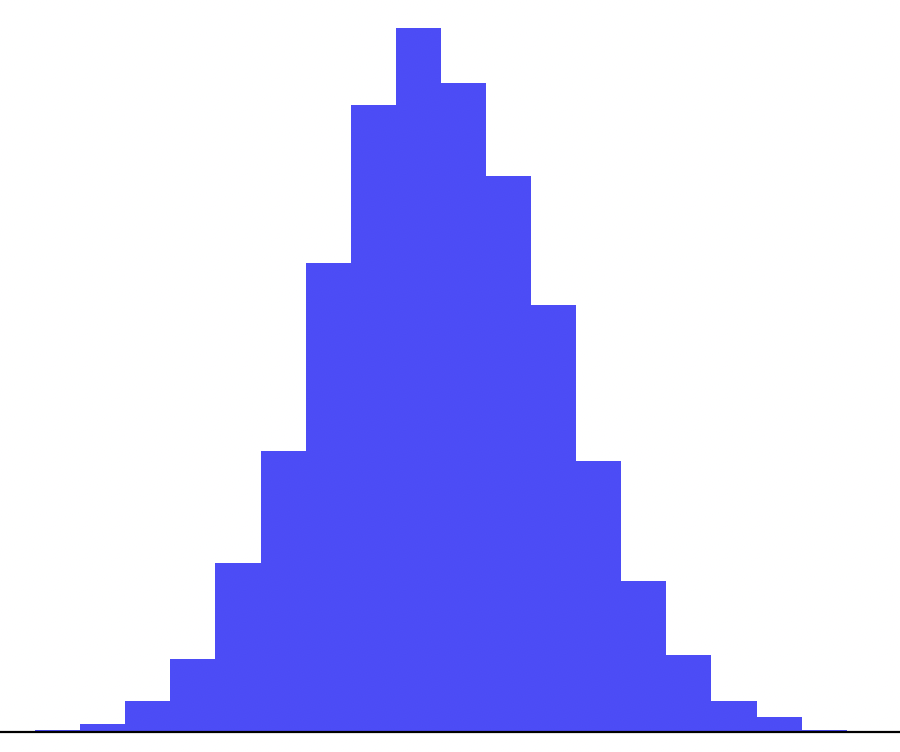
\includegraphics[width=8cm]{figures/hist2.png}};
  \node[draw=none] at (2.9,-0.2) {$X_{t+T}$};
\end{scope}

%%%%%%%%%%%%%%%%%%%%%%%%%%%%%%%%%%%%%
% Upper-right: slightly different ICDF
%%%%%%%%%%%%%%%%%%%%%%%%%%%%%%%%%%%%%
\begin{scope}[shift={(8,5)}]

  % ICDF definition
  \pgfmathdeclarefunction{Q}{1}{%
    \pgfmathparse{(#1)^3+0.2*(#1)+0.1}%
  }

  % Evaluate endpoints for dashed guides
  \pgfmathparse{Q(-1)} \let\Qminus\pgfmathresult
  \pgfmathparse{Q( 1)} \let\Qplus \pgfmathresult

  \begin{axis}[
    width=5.4cm, height=6.2cm,
    xmin=-1, xmax=1,
    ymin={min(0,\Qminus)-0.10*abs(\Qplus-\Qminus)},
    ymax={\Qplus + 0.10*abs(\Qplus-\Qminus)},
    axis x line=bottom,        % only the x-axis at the bottom
    axis y line=none,          % no y-axis
    axis line style={-},       % <-- ensure no arrowheads
    xlabel={$p$}, ylabel={},
    xtick=\empty, ytick=\empty,
    xlabel style={yshift=8pt},
    clip=false
  ]

    % ICDF curve
    \addplot[very thick, domain=-1:1, samples=400] ({x},{Q(x)});

    % short vertical ticks + labels at p=-1 and p=1
    \node[draw=none] at (0, -20)   (a) {$-1$};
    \node[draw=none] at (200, -20)   (b) {$1$};

    % dashed verticals from curve endpoints down to x-axis
    \draw[dashed] (axis cs:-1,-1.3) -- (axis cs:-1,\Qminus);
    \draw[dashed] (axis cs: 1,-1.3) -- (axis cs: 1,\Qplus);

  \end{axis}

\end{scope}

%%%%%%%%%%%%%%%%%%%%%%%%%%%%
% Arrows + labels
%%%%%%%%%%%%%%%%%%%%%%%%%%%%
\draw[arr, dashed] (3,7) -- (7,7);
\node[] at (5, 7.5) {Effective ICDF Timestepper};
\draw[arr] (0,3.7) -- (0,1.9);
\node[] at (2.5,2.9) {Sampling by Evaluating $F_t^{-1}$};
\draw[arr] (3,-1) -- (7,-1);
\node[] at (5, 0) {Particle Timestepper};
\draw[arr] (10.1,1.9) -- (10.1,3.7);
\node[] at (8,2.9) {Optimal Transport Map};

\end{tikzpicture}
\end{document}